% This file was created by tikzplotlib v0.9.1.
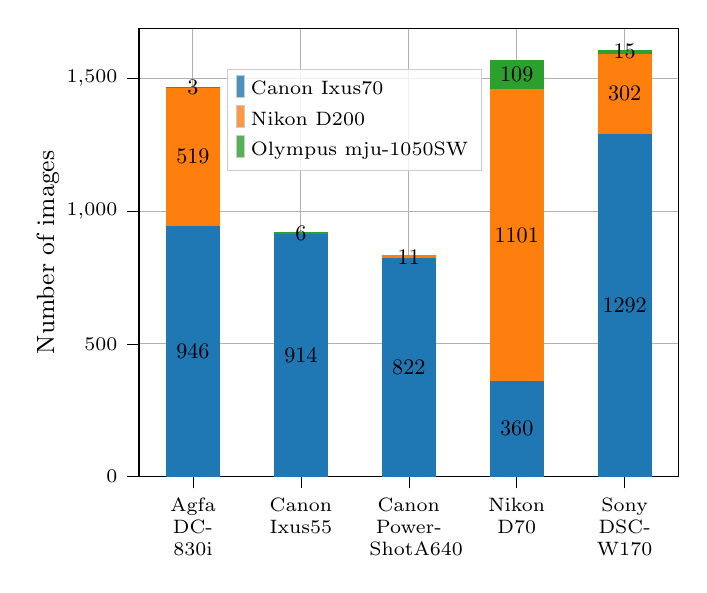
\begin{tikzpicture}

\definecolor{color0}{rgb}{0.12156862745098,0.466666666666667,0.705882352941177}
\definecolor{color1}{rgb}{1,0.498039215686275,0.0549019607843137}
\definecolor{color2}{rgb}{0.172549019607843,0.627450980392157,0.172549019607843}

\pgfplotsset{compat=1.11,
	/pgfplots/ybar legend/.style={
		/pgfplots/legend image code/.code={%
			\draw[##1,/tikz/.cd,yshift=-0.25em]
			(0cm,0cm) rectangle (3pt,0.8em);},
	}, every tick label/.append style={font=\scriptsize}
}

\begin{axis}[
legend cell align={left},
legend style={fill opacity=0.8, draw opacity=1, text opacity=1, at={(0.4,0.91)}, anchor=north, draw=white!80!black},
tick align=outside,
tick pos=left,
grid=major,
x grid style={white!69.0196078431373!black},
xmin=-0.5, xmax=4.5,
xtick style={color=black},
xtick={0,1,2,3,4},
xticklabel style={text width=1cm, align=center},
xticklabels={Agfa DC-830i, Canon Ixus55, Canon PowerShotA640, Nikon D70, Sony DSC-W170},
y grid style={white!69.0196078431373!black},
ymin=0, ymax=1689.45,
ytick style={color=black},
y label style={at={(axis description cs:-0.13,.5)},anchor=south},
ylabel={\small Number of images}
]
\draw[draw=none,fill=color0] (axis cs:-0.25,0) rectangle (axis cs:0.25,946);
\addlegendimage{ybar,ybar legend,draw=none,fill=color0};
\addlegendentry{\scriptsize Canon Ixus70}

\draw[draw=none,fill=color0] (axis cs:0.75,0) rectangle (axis cs:1.25,914);
\draw[draw=none,fill=color0] (axis cs:1.75,0) rectangle (axis cs:2.25,822);
\draw[draw=none,fill=color0] (axis cs:2.75,0) rectangle (axis cs:3.25,360);
\draw[draw=none,fill=color0] (axis cs:3.75,0) rectangle (axis cs:4.25,1292);
\draw[draw=none,fill=color1] (axis cs:-0.25,946) rectangle (axis cs:0.25,1465);
\addlegendimage{ybar,ybar legend,draw=none,fill=color1};
\addlegendentry{\scriptsize Nikon D200}

\draw[draw=none,fill=color1] (axis cs:0.75,0) rectangle (axis cs:1.25,0);
\draw[draw=none,fill=color1] (axis cs:1.75,822) rectangle (axis cs:2.25,833);
\draw[draw=none,fill=color1] (axis cs:2.75,360) rectangle (axis cs:3.25,1461);
\draw[draw=none,fill=color1] (axis cs:3.75,1292) rectangle (axis cs:4.25,1594);
\draw[draw=none,fill=color2] (axis cs:-0.25,1465) rectangle (axis cs:0.25,1468);
\addlegendimage{ybar,ybar legend,draw=none,fill=color2};
\addlegendentry{\scriptsize Olympus mju-1050SW}

\draw[draw=none,fill=color2] (axis cs:0.75,914) rectangle (axis cs:1.25,920);
\draw[draw=none,fill=color2] (axis cs:1.75,0) rectangle (axis cs:2.25,0);
\draw[draw=none,fill=color2] (axis cs:2.75,1461) rectangle (axis cs:3.25,1570);
\draw[draw=none,fill=color2] (axis cs:3.75,1594) rectangle (axis cs:4.25,1609);
\draw (axis cs:0,473) node[
  scale=0.8,
  text=black,
  rotate=0.0
]{946};
\draw (axis cs:1,457) node[
  scale=0.8,
  text=black,
  rotate=0.0
]{914};
\draw (axis cs:2,411) node[
  scale=0.8,
  text=black,
  rotate=0.0
]{822};
\draw (axis cs:3,180) node[
  scale=0.8,
  text=black,
  rotate=0.0
]{360};
\draw (axis cs:4,646) node[
  scale=0.8,
  text=black,
  rotate=0.0
]{1292};
\draw (axis cs:0,1205.5) node[
  scale=0.8,
  text=black,
  rotate=0.0
]{519};
\draw (axis cs:2,827.5) node[
  scale=0.8,
  text=black,
  rotate=0.0
]{11};
\draw (axis cs:3,910.5) node[
  scale=0.8,
  text=black,
  rotate=0.0
]{1101};
\draw (axis cs:4,1443) node[
  scale=0.8,
  text=black,
  rotate=0.0
]{302};
\draw (axis cs:0,1466.5) node[
  scale=0.8,
  text=black,
  rotate=0.0
]{3};
\draw (axis cs:1,917) node[
  scale=0.8,
  text=black,
  rotate=0.0
]{6};
\draw (axis cs:3,1515.5) node[
  scale=0.8,
  text=black,
  rotate=0.0
]{109};
\draw (axis cs:4,1601.5) node[
  scale=0.8,
  text=black,
  rotate=0.0
]{15};
\end{axis}

\end{tikzpicture}
